%%
%% Suspensions chapter
%%
%% Author:
%% Version:
%%
%\documentclass[color,cite,epsfig,12pt]{article}
%\usepackage{graphicx}
%\usepackage{placeins}
%\begin{document}
%%\bibliographystyle{unsrt} 



%%
%\vskip 3mm
%%
\subsection{Geometric anti-springs as seismic attenuation filters}
%%\subsection{Geometric anti-springs as seismic attenuation filters}
\label{sec:Gas_spring}
\vskip 2mm
An evolution of the Virgo mechanical filter to be used as vertical seismic noise  
suppression system, has been developed at Caltech~\cite{cella}, AEI and NIKHEF.
The anti-spring effect of this new technolgy is based on a particular geometry of the
elastic elements, the blades, mounted on a metallic disk and forming the so called 
\emph{Geometric Anti-Springs} (GAS) filter.
Seismic filters based on this effect have been successfully employed in the TAMA 
interferometer~\cite{tamaexperience} and now the GAS solution represents the baseline 
option for the optical components suspensions of the cryogenic and underground gravitational 
waves detector LCGT at Kamioka in Japan.

The GAS filter, shown in Fig.~\ref{fig:gas1}, consists of a set of radially arranged cantilever 
spring blades clamped at the base to a common frame disk and opposing each other via a central 
ring or keystone. 
\begin{figure}[htbp!]
\centering
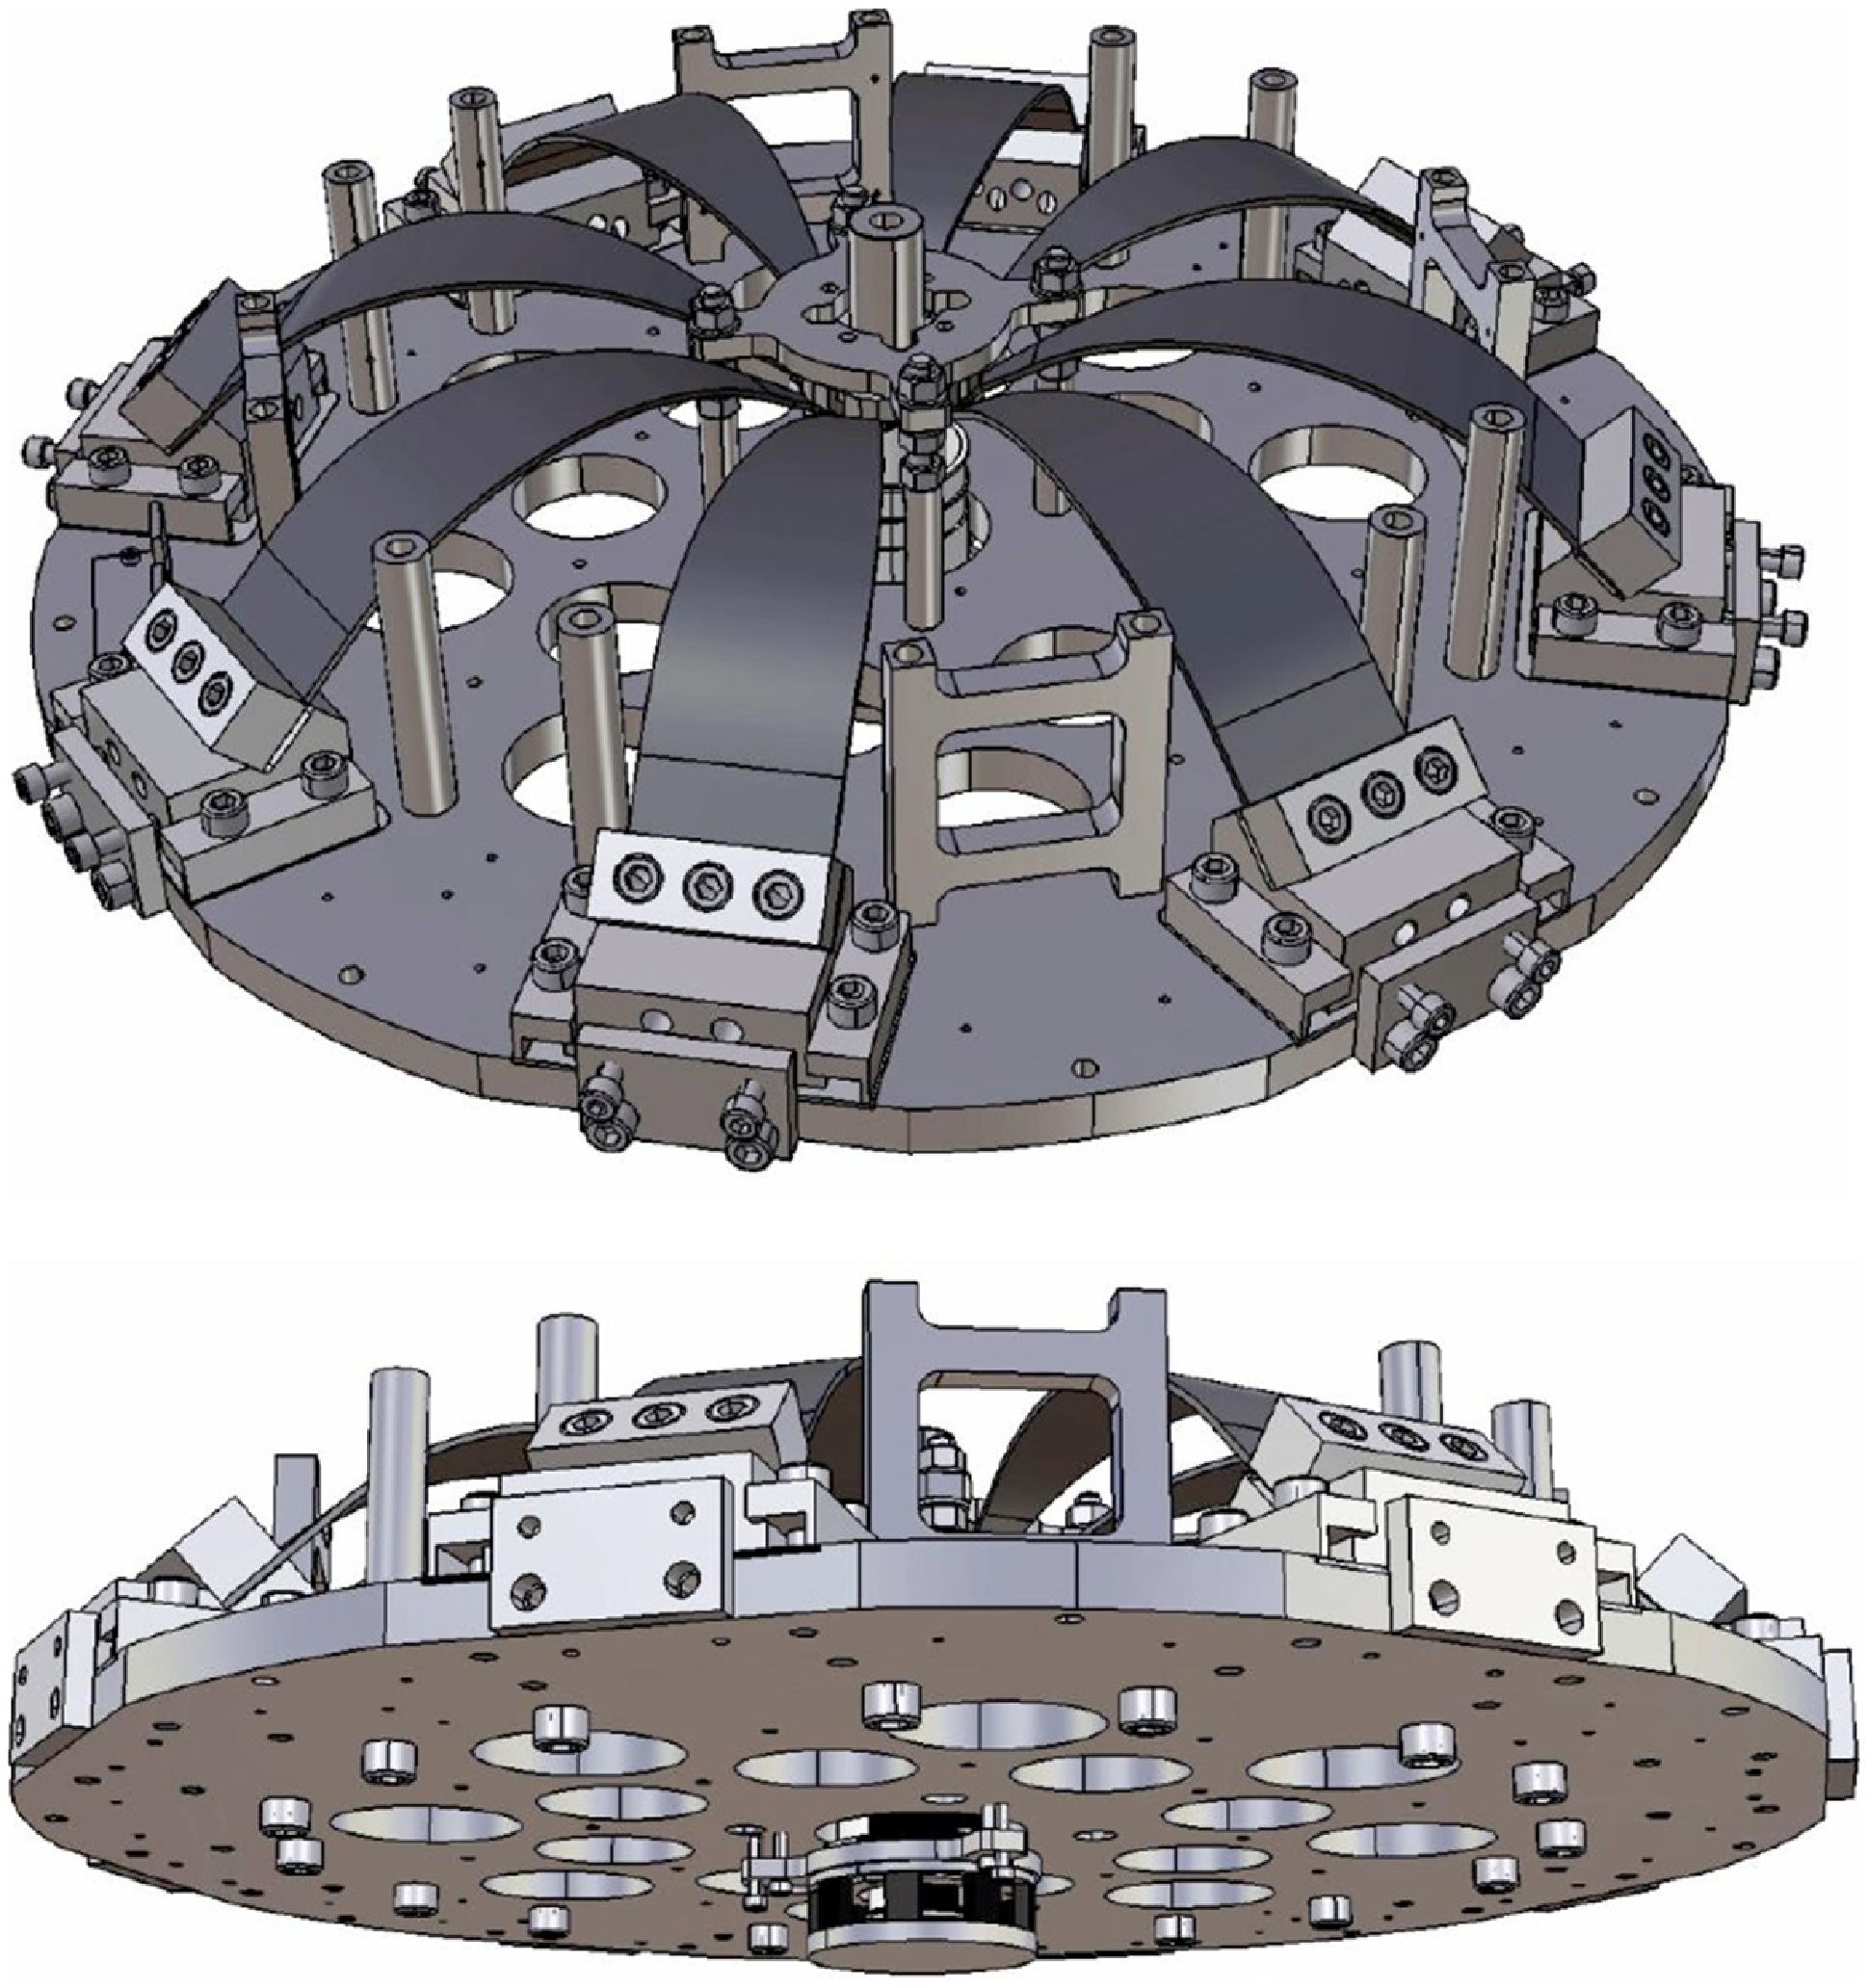
\includegraphics[width=6cm]{./Sec_Suspensions/Figures/gas1.pdf}
\caption{A 3D rendering view of a GAS filter used as seismic isolation system for the 10 m 
long interferometer at AEI Hannover. The same technology is used by the NIKHEF group for 
the the optical bench of the light injection in the interfrometer of Advanced Virgo. A voice coil actuator, visible on the bottom part of the figure, 
is located in the center of the filter.}
\label{fig:gas1}
\end{figure}

The blades are machined with a flat triangular shape while they become bended as soon as 
a suitable load is applied on their bases pushing the mechanical structure toward
the filter center. Since these elastic elements are compressed with a very high stress,
(up to 1.8 GPa) the material choice for their construction plays a fondamental role. To this 
purpose the Maraging steel ~\cite{Braccini2000} has been selected because it guarantees 
low creep noise level, low deformability and high thermal stability under high stress applied.
Each filter is an adjustable spring formed by a crown of curved cantilever blades compressed 
each against the other: the constrained radial stress creates an anti-spring effect 
(geometric anti-spring)~\cite{Bertolini} that allows a low effective stiffness to be achieved 
in the vertical direction when the nominal load is hung. 

The main features of the GAS filters are:
\begin{itemize}
\item{} Compact design with a limited number of mechanical elements;
\item{} UHV compatible;
\item{} Fast assembly and tuning;
\item{} Possibility to implement an active control (e.g.\ electro-magnetic antispring EMAS) 
with LVDT sensor and a voice coil actuator integrated into the design; 
\item{} Excellent attenuation performance when carefully tuned and operated under vacuum.
\end{itemize}

A photo of a geometric anti-spring assembled at NIKHEF and an LCGT prototype is shown 
in Fig.~\ref{fig:gas_nikhef}.

\begin{figure}[htbp!]
\centering
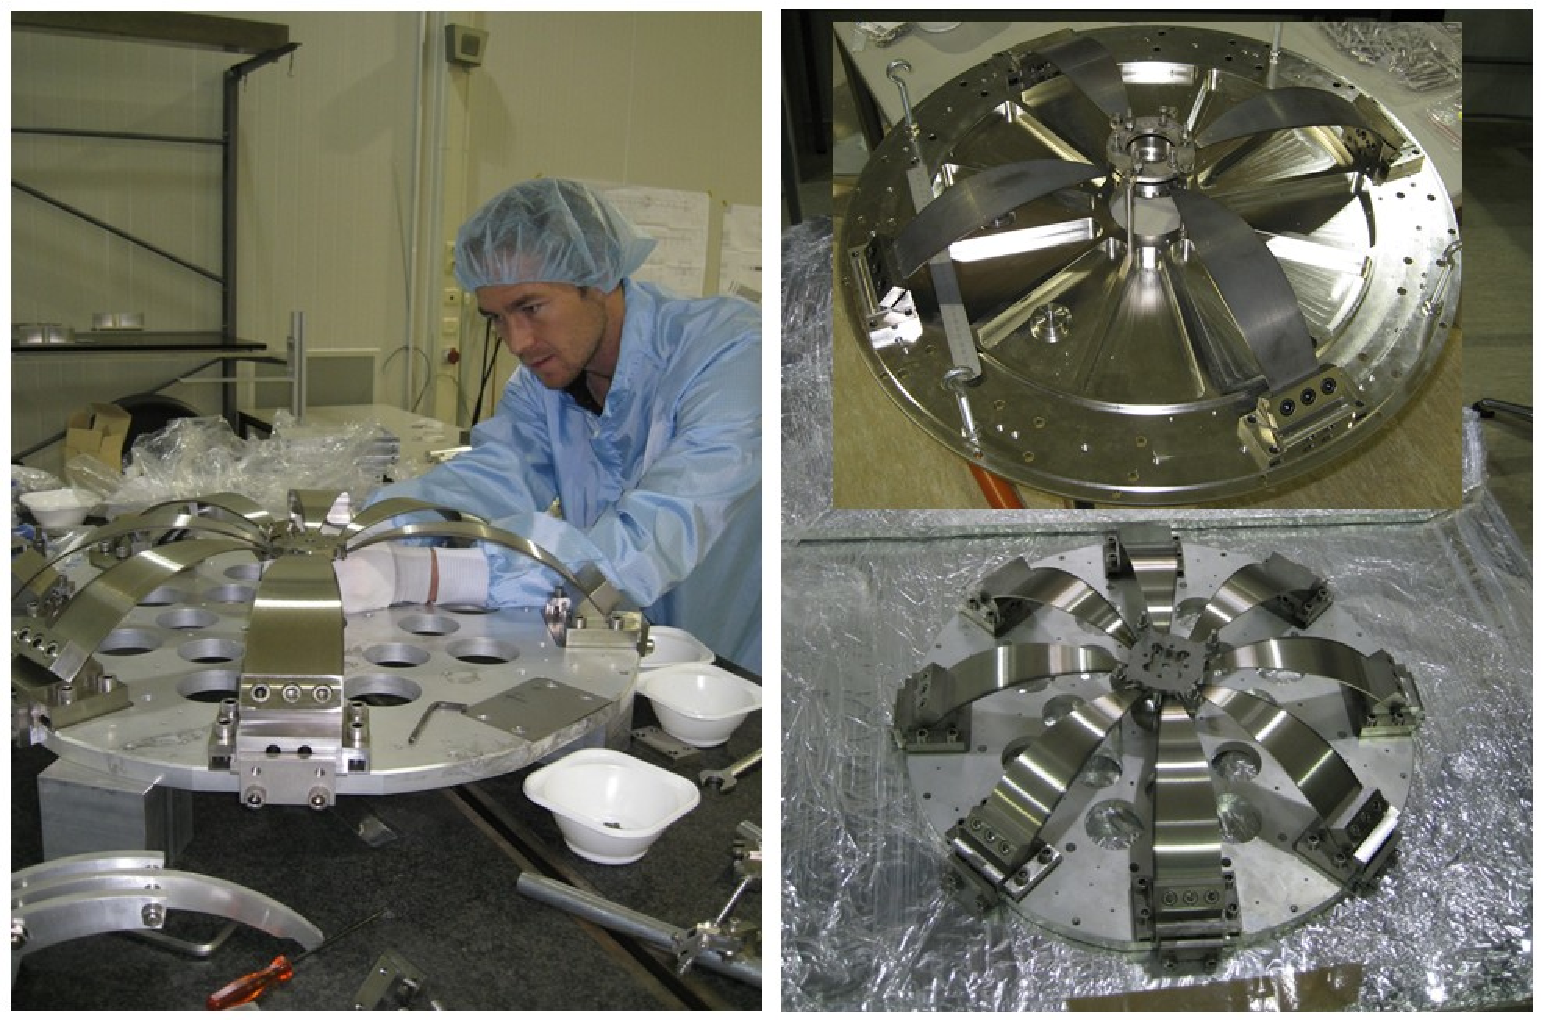
\includegraphics[width=9cm]{./Sec_Suspensions/Figures/gas_nikhef.pdf}
\caption{Pictures of the GAS filter prototypes. The left and top right panels
show a filter built and tested at NIKHEF for the Virgo external injection bench ~\cite{nikhef}.
The bottom right panel shows a prototype for LCGT suspension.}
\label{fig:gas_nikhef}
\end{figure}

A vertical cut-off frequency down to 0.30\,Hz have been obtained through a fine mechanical 
adjustment of the compression rate while longer natural period can be achieved by applying 
positive feedback (the so-called electro-magnetic anti-spring - EMAS). 
The performance of a GAS filter is shown in Fig. \ref{fig:hamsassensv} where a comparison 
between the model and the measurements performed using a system with three blades is reported.
In the plot a seismic attenuation performance of -60 dB at about 10 Hz is visible
while an isolation level down to -80 dB (at frequncy higher than 10 Hz) can be reached by using 
a set of overcompensating wands ~\cite{stochino}.

\begin{figure}[htbp!]
\centering
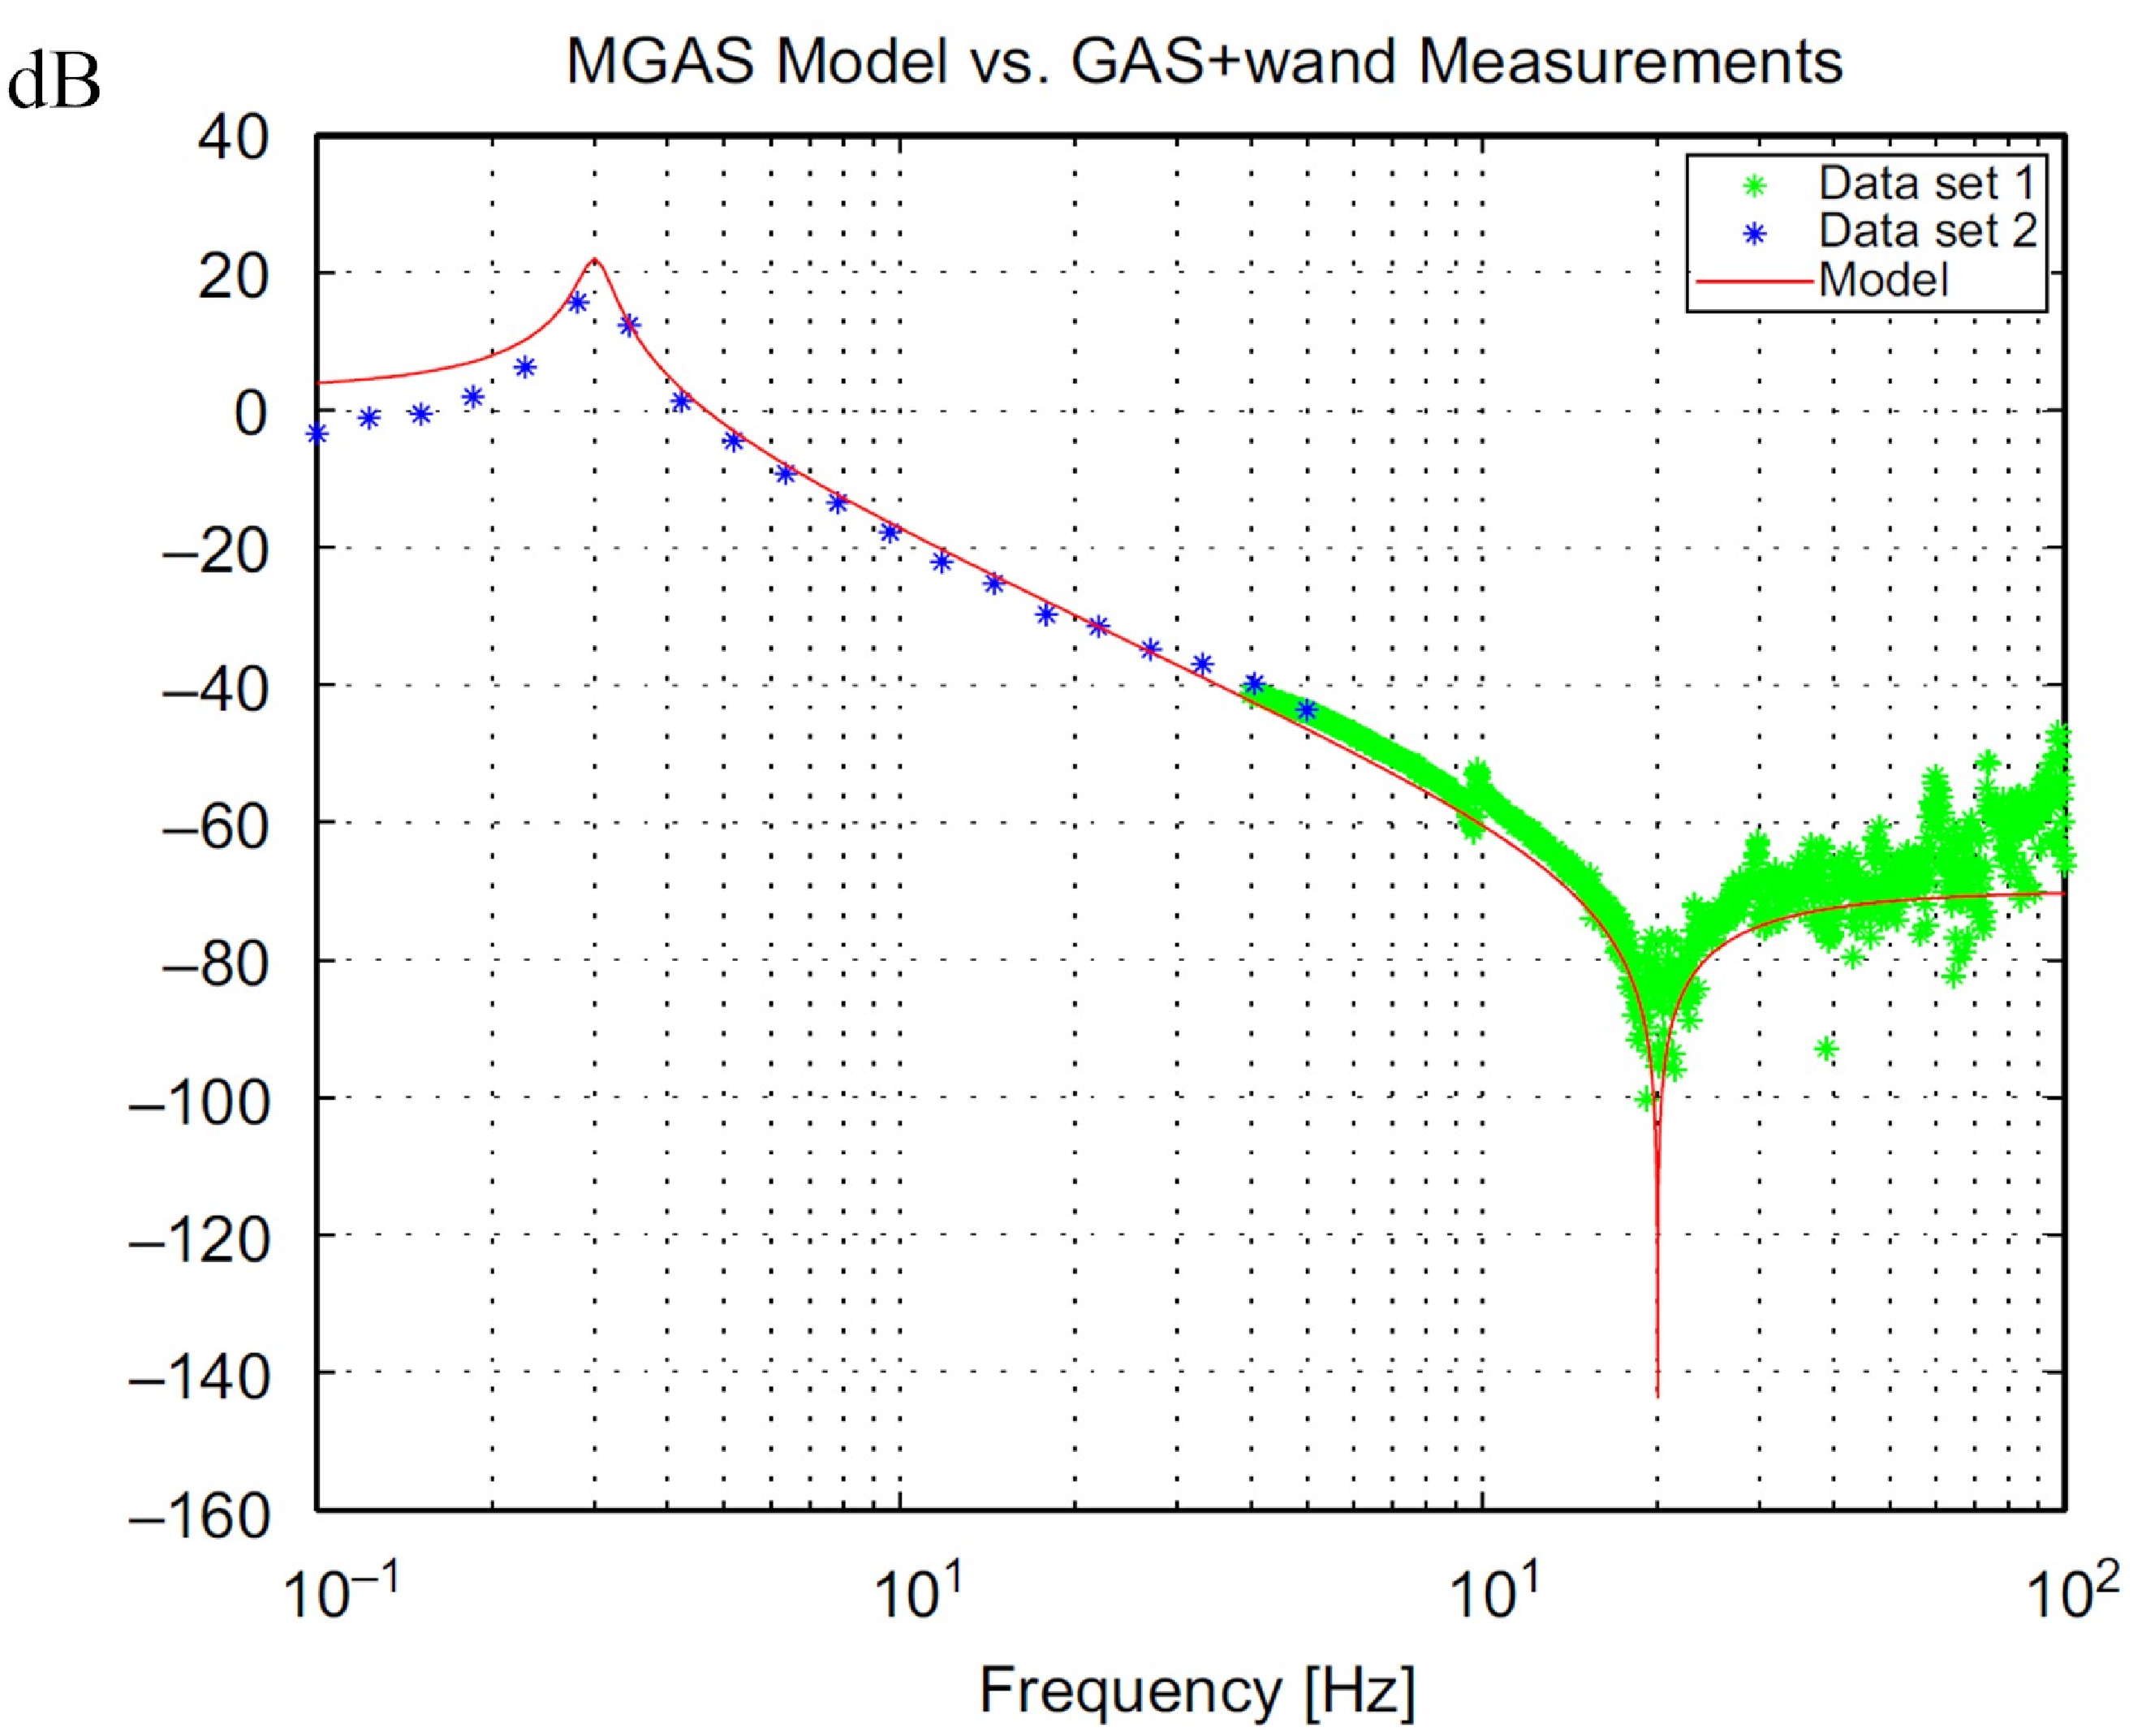
\includegraphics[width=10cm]{./Sec_Suspensions/Figures/hamsassensv.pdf}
\caption{Vertical attenuation performance of a GAS filter with overcompensating 
wands \cite{stochino}}
\label{fig:hamsassensv}
\end{figure}

Finite element analysis (FEA)~\cite{Hennes} and a measurements campaign on a GAS filter 
prototype are in progress in AEI Hannover and NIKHEF. They provide valuable input 
for the GAS filter fine tuning and its behaviour as a function of the environmental temperature.  
Detailed studies on a filter prototype for LCGT project and with different blades shapes 
are also in progress at NIKHEF.
 

%\end{document}